\section{Introduction}

\begin{figure}[!t]
\centering
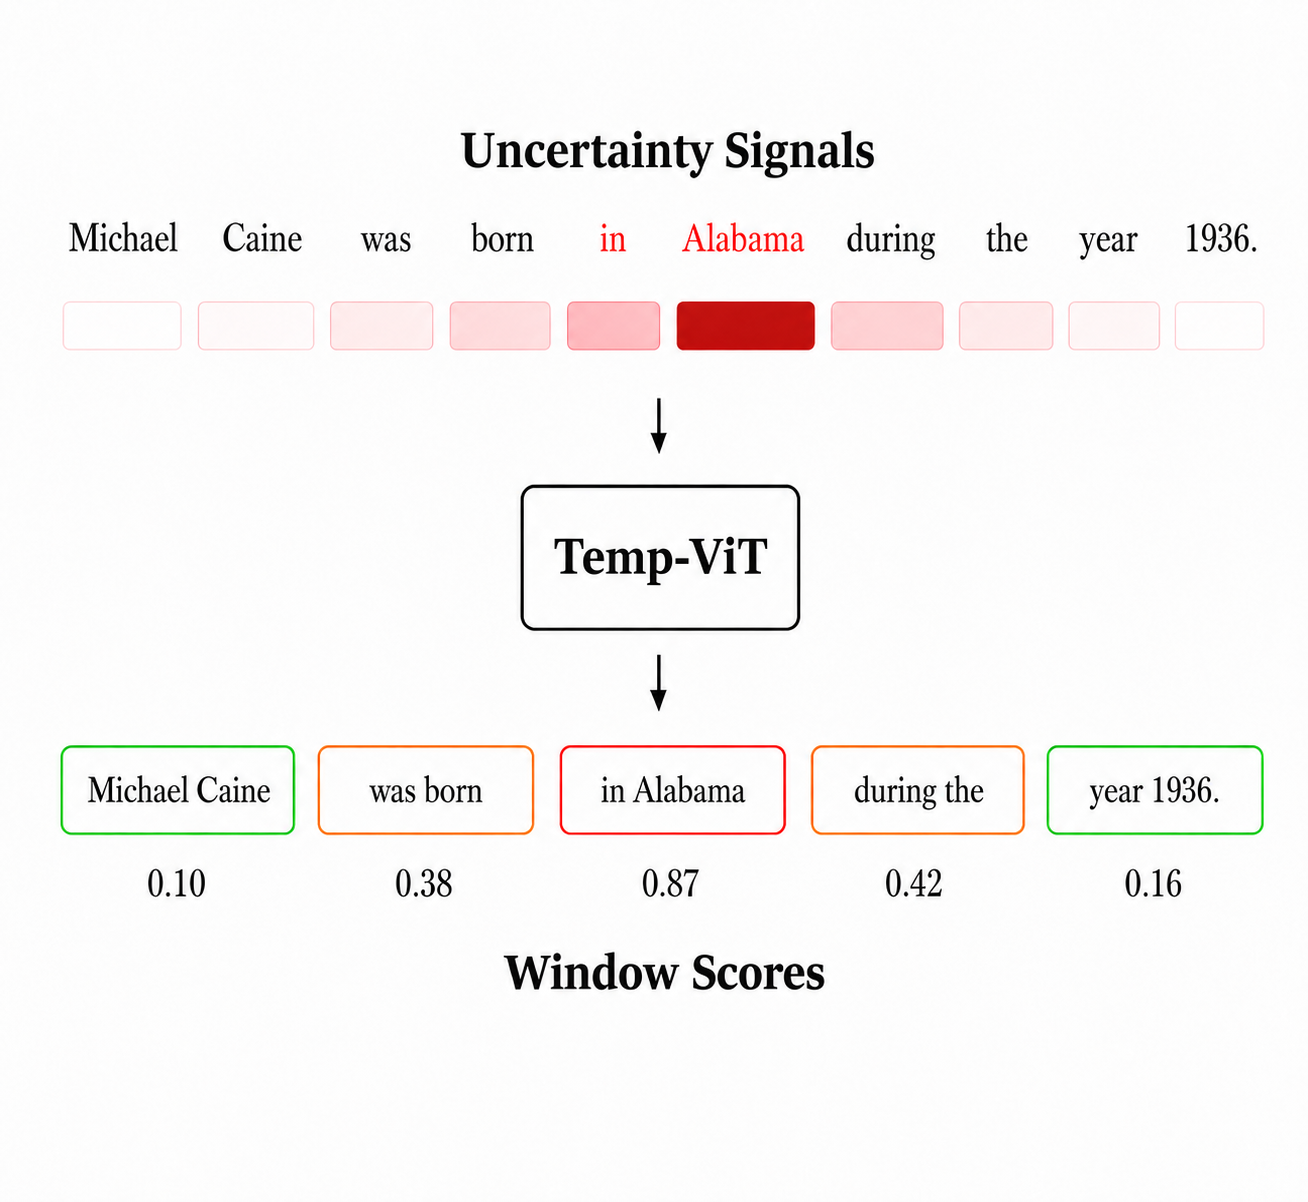
\includegraphics[width=\linewidth]{figs/tpe_example.png}
\caption{TPE on a generated sentence: per-token uncertainty signals from
the LLM's hidden states (top) are read by TPE and aggregated into
per-window hallucination scores (bottom), localizing the unsupported
span \emph{``in Alabama''} without per-token labels.}
\label{fig:tpe_example}
\end{figure}


\paragraph{Why this matters.}
Recent progress in large language models has demonstrated impressive capabilities in generating long-form answers across retrieval-augmented generation, biographies, and explanatory tasks.
However, their growing use also raises concerns about reliability, because fluent outputs can contain localized factual errors that are difficult to notice. A useful hallucination detector should identify where unreliable content appears, not just whether the full response is hallucinated. This distinction matters for retrieval-augmented answers, biographies, and long explanations, where a single unsupported span can be hidden inside otherwise correct text
\citep{niu2024ragtruth,min2023,wei2024}.

\paragraph{What current methods leave open.}
Confidence-based methods estimate uncertainty from sequence probabilities,
entropy, or related token statistics, but they do not directly model semantic
equivalence and often degrade on long-form generations
\citep{malinin2021uncertainty,duan2024shifting,schweighofer2025rethinking}.
Sampling-based methods compare several generations, and verifier pipelines
decompose responses into claims and check them with external systems
\citep{kuhn2023semantic,lin2024generating,jiang2024,manakul2023,min2023,zhao2024}.
These methods can be accurate, but repeated sampling, retrieval, or LLM-based
judging is expensive when applied across long passages. Mechanistic methods avoid
extra LLM calls by inspecting hidden states of the generating model
\citep{azaria2023,marks2023,liu2024,ji2024}, but each family hits a different
wall. Fixed layer-token probes are cheap but miss uncertainty signals that move
across layers, positions, models, and tasks \citep{kadavath2022,orgad2024}.
Full-response activation-map probes capture more distributed signal, but pooling
a whole response into one representation produces a sequence-level score and
forces a tradeoff between speed and accuracy as outputs grow longer
\citep{barshalom2025}. The common workaround is to extract claims, classify each
claim, and broadcast the verdict to the claim's text span, but this ignores
pre-span, post-span, and boundary evidence in the surrounding generation
\citep{snyder2024,he2024}.

\paragraph{Our approach and contributions.}
We recast mechanistic hallucination detection as weakly supervised temporal
localization (WSTL), borrowing from video understanding: a video model localizes
an action from clip-level labels without per-frame supervision
\citep{pilhyeonlee2021}. We treat hidden-state activations as a temporal sequence
over the generated token axis. Each instance is a fixed-length activation window
whose layer-token plane preserves local structure across layers and nearby
tokens. Figure~\ref{fig:tpe_example} shows the motivation for this windowed view:
hallucination evidence can appear before the unsupported tokens and influence
the hallucinated span. Based on this representation, we build Temporal Perception
Encoder (TPE): a Perception Encoder over local layer-token activation windows
paired with a temporal head that propagates window-level uncertainty evidence
across the response \citep{bolya2025perceptionencoder,albertgu2024}. Concretely,
we contribute:
\begin{enumerate}
    \item We formulate mechanistic hallucination detection as weakly supervised
    temporal localization over hidden-state activation windows, enabling predictions
    as granular as token level from claim labels.

    \item We propose TPE, a windowed hallucination detection model that encodes local
    layer-token activations with a Perception Encoder and propagates hallucination signals with
    a temporal head. We train it with a three-stage weak-supervision framework that learns
    hallucination activation patterns with claim labels, localizes responsible windows with
    top-$k$ MIL, and refines boundary behavior across neighboring correct and
    hallucinated claims.

    \item We demonstrate granular long-form hallucination localization on
    biographical generation, open-ended factual QA, and retrieval-augmented QA
    when using claim-level labels for training. 
    We also show it outperforms other methods on short-form and long-form QA, machine translation, and math
    even when using weaker sequence-level labels.
\end{enumerate}
